
%
\documentclass[journal]{IEEEtran}
%
% If IEEEtran.cls has not been installed into the LaTeX system files,
% manually specify the path to it like:
% \documentclass[journal]{../sty/IEEEtran}




% *** MISC UTILITY PACKAGES ***
%
%\usepackage{ifpdf}
% Heiko Oberdiek's ifpdf.sty is very useful if you need conditional
% compilation based on whether the output is pdf or dvi.
% usage:
% \ifpdf
%   % pdf code
% \else
%   % dvi code
% \fi
% The latest version of ifpdf.sty can be obtained from:
% http://www.ctan.org/tex-archive/macros/latex/contrib/oberdiek/
% Also, note that IEEEtran.cls V1.7 and later provides a builtin
% \ifCLASSINFOpdf conditional that works the same way.
% When switching from latex to pdflatex and vice-versa, the compiler may
% have to be run twice to clear warning/error messages.


% *** CITATION PACKAGES ***
%
%\usepackage{cite}
% cite.sty was written by Donald Arseneau
% V1.6 and later of IEEEtran pre-defines the format of the cite.sty package
% \cite{} output to follow that of IEEE. Loading the cite package will
% result in citation numbers being automatically sorted and properly
% "compressed/ranged". e.g., [1], [9], [2], [7], [5], [6] without using
% cite.sty will become [1], [2], [5]--[7], [9] using cite.sty. cite.sty's
% \cite will automatically add leading space, if needed. Use cite.sty's
% noadjust option (cite.sty V3.8 and later) if you want to turn this off
% such as if a citation ever needs to be enclosed in parenthesis.
% cite.sty is already installed on most LaTeX systems. Be sure and use
% version 4.0 (2003-05-27) and later if using hyperref.sty. cite.sty does
% not currently provide for hyperlinked citations.
% The latest version can be obtained at:
% http://www.ctan.org/tex-archive/macros/latex/contrib/cite/
% The documentation is contained in the cite.sty file itself.


% *** GRAPHICS RELATED PACKAGES ***
%
\ifCLASSINFOpdf
  % \usepackage[pdftex]{graphicx}
  % declare the path(s) where your graphic files are
  % \graphicspath{{../pdf/}{../jpeg/}}
  % and their extensions so you won't have to specify these with
  % every instance of \includegraphics
  % \DeclareGraphicsExtensions{.pdf,.jpeg,.png}
\else
  % or other class option (dvipsone, dvipdf, if not using dvips). graphicx
  % will default to the driver specified in the system graphics.cfg if no
  % driver is specified.
  % \usepackage[dvips]{graphicx}
  % declare the path(s) where your graphic files are
  % \graphicspath{{../eps/}}
  % and their extensions so you won't have to specify these with
  % every instance of \includegraphics
  % \DeclareGraphicsExtensions{.eps}
\fi




% *** MATH PACKAGES ***
%
%\usepackage[cmex10]{amsmath}
% A popular package from the American Mathematical Society that provides
% many useful and powerful commands for dealing with mathematics. If using
% it, be sure to load this package with the cmex10 option to ensure that
% only type 1 fonts will utilized at all point sizes. Without this option,
% it is possible that some math symbols, particularly those within
% footnotes, will be rendered in bitmap form which will result in a
% document that can not be IEEE Xplore compliant!
%
% Also, note that the amsmath package sets \interdisplaylinepenalty to 10000
% thus preventing page breaks from occurring within multiline equations. Use:
%\interdisplaylinepenalty=2500
% after loading amsmath to restore such page breaks as IEEEtran.cls normally
% does. amsmath.sty is already installed on most LaTeX systems. The latest
% version and documentation can be obtained at:
% http://www.ctan.org/tex-archive/macros/latex/required/amslatex/math/





% *** SPECIALIZED LIST PACKAGES ***
%
%\usepackage{algorithmic}
% algorithmic.sty was written by Peter Williams and Rogerio Brito.
% This package provides an algorithmic environment fo describing algorithms.
% You can use the algorithmic environment in-text or within a figure
% environment to provide for a floating algorithm. Do NOT use the algorithm
% floating environment provided by algorithm.sty (by the same authors) or
% algorithm2e.sty (by Christophe Fiorio) as IEEE does not use dedicated
% algorithm float types and packages that provide these will not provide
% correct IEEE style captions. The latest version and documentation of
% algorithmic.sty can be obtained at:
% http://www.ctan.org/tex-archive/macros/latex/contrib/algorithms/
% There is also a support site at:
% http://algorithms.berlios.de/index.html
% Also of interest may be the (relatively newer and more customizable)
% algorithmicx.sty package by Szasz Janos:
% http://www.ctan.org/tex-archive/macros/latex/contrib/algorithmicx/




% *** ALIGNMENT PACKAGES ***
%
%\usepackage{array}
% Frank Mittelbach's and David Carlisle's array.sty patches and improves
% the standard LaTeX2e array and tabular environments to provide better
% appearance and additional user controls. As the default LaTeX2e table
% generation code is lacking to the point of almost being broken with
% respect to the quality of the end results, all users are strongly
% advised to use an enhanced (at the very least that provided by array.sty)
% set of table tools. array.sty is already installed on most systems. The
% latest version and documentation can be obtained at:
% http://www.ctan.org/tex-archive/macros/latex/required/tools/


% IEEEtran contains the IEEEeqnarray family of commands that can be used to
% generate multiline equations as well as matrices, tables, etc., of high
% quality.




% *** SUBFIGURE PACKAGES ***
%\ifCLASSOPTIONcompsoc
%  \usepackage[caption=false,font=normalsize,labelfont=sf,textfont=sf]{subfig}
%\else
%  \usepackage[caption=false,font=footnotesize]{subfig}
%\fi
% subfig.sty, written by Steven Douglas Cochran, is the modern replacement
% for subfigure.sty, the latter of which is no longer maintained and is
% incompatible with some LaTeX packages including fixltx2e. However,
% subfig.sty requires and automatically loads Axel Sommerfeldt's caption.sty
% which will override IEEEtran.cls' handling of captions and this will result
% in non-IEEE style figure/table captions. To prevent this problem, be sure
% and invoke subfig.sty's "caption=false" package option (available since
% subfig.sty version 1.3, 2005/06/28) as this is will preserve IEEEtran.cls
% handling of captions.
% Note that the Computer Society format requires a larger sans serif font
% than the serif footnote size font used in traditional IEEE formatting
% and thus the need to invoke different subfig.sty package options depending
% on whether compsoc mode has been enabled.
%
% The latest version and documentation of subfig.sty can be obtained at:
% http://www.ctan.org/tex-archive/macros/latex/contrib/subfig/



% *** FLOAT PACKAGES ***
%
%\usepackage{fixltx2e}
% fixltx2e, the successor to the earlier fix2col.sty, was written by
% Frank Mittelbach and David Carlisle. This package corrects a few problems
% in the LaTeX2e kernel, the most notable of which is that in current
% LaTeX2e releases, the ordering of single and double column floats is not
% guaranteed to be preserved. Thus, an unpatched LaTeX2e can allow a
% single column figure to be placed prior to an earlier double column
% figure. The latest version and documentation can be found at:
% http://www.ctan.org/tex-archive/macros/latex/base/


%\usepackage{stfloats}
% stfloats.sty was written by Sigitas Tolusis. This package gives LaTeX2e
% the ability to do double column floats at the bottom of the page as well
% as the top. (e.g., "\begin{figure*}[!b]" is not normally possible in
% LaTeX2e). It also provides a command:
%\fnbelowfloat
% to enable the placement of footnotes below bottom floats (the standard
% LaTeX2e kernel puts them above bottom floats). This is an invasive package
% which rewrites many portions of the LaTeX2e float routines. It may not work
% with other packages that modify the LaTeX2e float routines. The latest
% version and documentation can be obtained at:
% http://www.ctan.org/tex-archive/macros/latex/contrib/sttools/
% Do not use the stfloats baselinefloat ability as IEEE does not allow
% \baselineskip to stretch. Authors submitting work to the IEEE should note
% that IEEE rarely uses double column equations and that authors should try
% to avoid such use. Do not be tempted to use the cuted.sty or midfloat.sty
% packages (also by Sigitas Tolusis) as IEEE does not format its papers in
% such ways.
% Do not attempt to use stfloats with fixltx2e as they are incompatible.
% Instead, use Morten Hogholm'a dblfloatfix which combines the features
% of both fixltx2e and stfloats:
%
% \usepackage{dblfloatfix}
% The latest version can be found at:
% http://www.ctan.org/tex-archive/macros/latex/contrib/dblfloatfix/




%\ifCLASSOPTIONcaptionsoff
%  \usepackage[nomarkers]{endfloat}
% \let\MYoriglatexcaption\caption
% \renewcommand{\caption}[2][\relax]{\MYoriglatexcaption[#2]{#2}}
%\fi
% endfloat.sty was written by James Darrell McCauley, Jeff Goldberg and 
% Axel Sommerfeldt. This package may be useful when used in conjunction with 
% IEEEtran.cls'  captionsoff option. Some IEEE journals/societies require that
% submissions have lists of figures/tables at the end of the paper and that
% figures/tables without any captions are placed on a page by themselves at
% the end of the document. If needed, the draftcls IEEEtran class option or
% \CLASSINPUTbaselinestretch interface can be used to increase the line
% spacing as well. Be sure and use the nomarkers option of endfloat to
% prevent endfloat from "marking" where the figures would have been placed
% in the text. The two hack lines of code above are a slight modification of
% that suggested by in the endfloat docs (section 8.4.1) to ensure that
% the full captions always appear in the list of figures/tables - even if
% the user used the short optional argument of \caption[]{}.
% IEEE papers do not typically make use of \caption[]'s optional argument,
% so this should not be an issue. A similar trick can be used to disable
% captions of packages such as subfig.sty that lack options to turn off
% the subcaptions:
% For subfig.sty:
% \let\MYorigsubfloat\subfloat
% \renewcommand{\subfloat}[2][\relax]{\MYorigsubfloat[]{#2}}
% However, the above trick will not work if both optional arguments of
% the \subfloat command are used. Furthermore, there needs to be a
% description of each subfigure *somewhere* and endfloat does not add
% subfigure captions to its list of figures. Thus, the best approach is to
% avoid the use of subfigure captions (many IEEE journals avoid them anyway)
% and instead reference/explain all the subfigures within the main caption.
% The latest version of endfloat.sty and its documentation can obtained at:
% http://www.ctan.org/tex-archive/macros/latex/contrib/endfloat/
%
% The IEEEtran \ifCLASSOPTIONcaptionsoff conditional can also be used
% later in the document, say, to conditionally put the References on a 
% page by themselves.




% correct bad hyphenation here
\hyphenation{op-tical net-works semi-conduc-tor}
\usepackage{graphicx}
\usepackage{subfloat}
\usepackage{subfigure}
\usepackage{subfig}
\usepackage{color}
\usepackage{amsmath}
\usepackage{amsfonts}
\usepackage{amssymb}
\usepackage{multirow}
\usepackage{algorithm}
\usepackage{algorithmicx}
\usepackage{algpseudocode}
\usepackage{amsmath}
\usepackage{graphics}
\usepackage{epsfig}
\usepackage{CJK}
\usepackage{amsmath}
\usepackage{caption}





\usepackage[font=small,labelsep=period]{caption}
\captionsetup{%
  figurename=Fig.,
  tablename=Table
  }

\begin{document}
%
% paper title
% can use linebreaks \\ within to get better formatting as desired
% Do not put math or special symbols in the title.
\title{ Learning and Recognizing 3D Objects without Manual Interference by a Self-taught Vision System}




\author{\IEEEauthorblockN{Ren C. Luo\IEEEauthorrefmark{1},
and Po-Yu Chuang\IEEEauthorrefmark{2},
}

\IEEEauthorblockA{\IEEEauthorrefmark{1} \IEEEauthorrefmark{2}Electrical Engineering Department, National
Taiwan University, Taipei, Taiwan 106}

}


\IEEEtitleabstractindextext{%
\begin{abstract}
Vision systems for 3D object recognition are widely applied on industrial robot arm recent years. Conventionally, vision, learning approach, and robot arm are separated into three different systems, so learning approach can only learn the distributions of input data, but cannot refine qualities of input and output without manual interference. Therefore, it may cause misfiring performance by erratic input or sustainable growth database. In this paper, we propose an intelligent vision system for 3D object recognition which is able to automatically construct and refine model for 3D object recognition without any manual interference. Although 2D images and rotation angles of robot arm are different domains, we model 3D objects by multiple 2D images and rotation angles, and information from different domains are integrated by a Hierarchical-Deep (HD) model with parallel branch. The model hierarchically extracts information by domains and levels. The parallel branch distinct labeled and unlabeled data to avoid performance drag by sustainable growth of unlabeled input. The relationships between label and unlabeled data are learned by proposed self-taught approach. The experimental results show the feasibility of proposed structure that can transfer knowledge in different domains with limited prior knowledge, and complete assigned task by only modeling the relation between input and output.

\end{abstract}

% Note that keywords are not normally used for peerreview papers.
\begin{IEEEkeywords}
industrial automation, machine vision, object recognition, Hierarchical-Deep model
\end{IEEEkeywords}}



% make the title area
\maketitle


% To allow for easy dual compilation without having to reenter the
% abstract/keywords data, the \IEEEtitleabstractindextext text will
% not be used in maketitle, but will appear (i.e., to be "transported")
% here as \IEEEdisplaynontitleabstractindextext when the compsoc 
% or transmag modes are not selected <OR> if conference mode is selected 
% - because all conference papers position the abstract like regular
% papers do.
\IEEEdisplaynontitleabstractindextext
% \IEEEdisplaynontitleabstractindextext has no effect when using
% compsoc or transmag under a non-conference mode.







% For peer review papers, you can put extra information on the cover
% page as needed:
% \ifCLASSOPTIONpeerreview
% \begin{center} \bfseries EDICS Category: 3-BBND \end{center}
% \fi
%
% For peerreview papers, this IEEEtran command inserts a page break and
% creates the second title. It will be ignored for other modes.
\IEEEpeerreviewmaketitle



\section{Introduction}


% The very first letter is a 2 line initial drop letter followed
% by the rest of the first word in caps.
% 
% form to use if the first word consists of a single letter:
% \IEEEPARstart{A}{demo} file is ....
% 
% form to use if you need the single drop letter followed by
% normal text (unknown if ever used by IEEE):
% \IEEEPARstart{A}{}demo file is ....
% 
% Some journals put the first two words in caps:
% \IEEEPARstart{T}{his demo} file is ....
% 
% Here we have the typical use of a "T" for an initial drop letter
% and "HIS" in caps to complete the first word.
\IEEEPARstart{R}{obot} arm with vision have been widely applied in automatic industrial production line in recent years [1-4]. New hurdles of conventional vision system arise due to rise of consumer electronic market. The components in assembling production line become small volume but large variety. The types of components are also changed rapidly because of short product life cycle. These conditions are tough for conventional vision system. Model-based recognition methods are commonly used in present industrial applications. The performance is mainly related to the manually labeled data. These manual works not only increase the labor cost, but also point out the dilemma of present vision-based robot is unable to automatically adapt to various assignments, and growing database.

Therefore, we propose an intelligent system which is able to handle sustainable growth of unlabeled input, and refine existed model without any manual interference. The situation of this paper is that we only provide target face of 3D objects which are intended to be placed on top by robot arm, but the other faces of 3D objects are unknown. The only prior knowledge is target faces, and inputs are arbitrary objects with random faces on top. The input of system is 2D image, and output is rotation angle of robot arm in Cartesian. Since input and output are different domains, the traditional single layer models [5,6] which end in a linear or kernel classifier is not enough. We introduced a \textit{\textbf{Hierarchical-Deep(HD)}} model[7] to tackle the problems. 

The learning of HD model achieves dramatically success recent years. Hinton et al. [7] proposed deep structure learning which hidden layers are formed by lower level feature to higher level hierarchically, and had been successfully applied on different research fields [8-11]. The proposed HD model is constructed by four layers:\textbf{Feature}, \textbf{Descriptor}, \textbf{Object} and \textbf{RotationAngle}. Being an automatic system, the ability which could "infer" latent edges between labeled and unlabeled data is needed. Latent edge means two variables in different layers exist an edge in graph model if prior data is sufficient, but, in our case, system only have small amount of prior data. Hence, there are many latent edges which are waiting to be revealed through learning process. 

The most challenge part is that the appearance of different faces of a single object might be quite different, so we design three modules to tackle self-taught problem. Firstly, we design a probabilistic based image descriptor. Although many methods [12-16] provide high quality performance by extracting sparse features, the sparse feature is not compact on inferring latent edges. The sparse feature only model strong features of observed face, but most of faces is unknown in our case. We need a descriptor which can provide sufficient information for inference, but still retain scale- and rotation-invariant. Proposed probabilistic based descriptor is established based on the \textit{\textbf{Markov Logic Network (MLN)}} [17-20]. MLN is an approach combines first-order logic and probabilistic graphical model. First-order logic enables compactly representing the neighborhood of feature points. Probabilistic graphical model can reveal latent edges by proper inference method, and also handle the uncertainty.  

Secondly, transfer information module is tailored to handle unlabeled data. Transfer information module is realized by Self-taught Clustering algorithm [21]. Self-taught Clustering algorithm is a transfer learning method [22-26] which is built for enhancing model through large amount of auxiliary unlabeled data. The input face can be considered auxiliary unlabeled data, and find co-cluster between prior faces in the dataset. The distribution of co-cluster is further utilized to infer the possible rotation angle for robot arm, and robot arm will rotate target object from input face to output face. Finally, the validation module is an eye-to-hand camera which used to validate the error between the output face and desired target. Then, the validation module returns the error to the model in order to refine the existed model. Through these three modules, proposed system can automatically learn the relations between input images and corresponding rotation angles with only labeled the target face of each object.

In this paper, we start with briefly overview of system design and structure in section 2. The MLN-based descriptor for recognizing object is described in section 3. Section 4 introduces how to model the proposed hierarchical networks, and learn by self-taught learning. Then, we compare the performance of proposed system with several states of development in section 5. Finally, reviewing performance and conclusions are presented in final section.


\begin{figure}[!t]
\begin{center}
%\subfigure[System architecture]{}
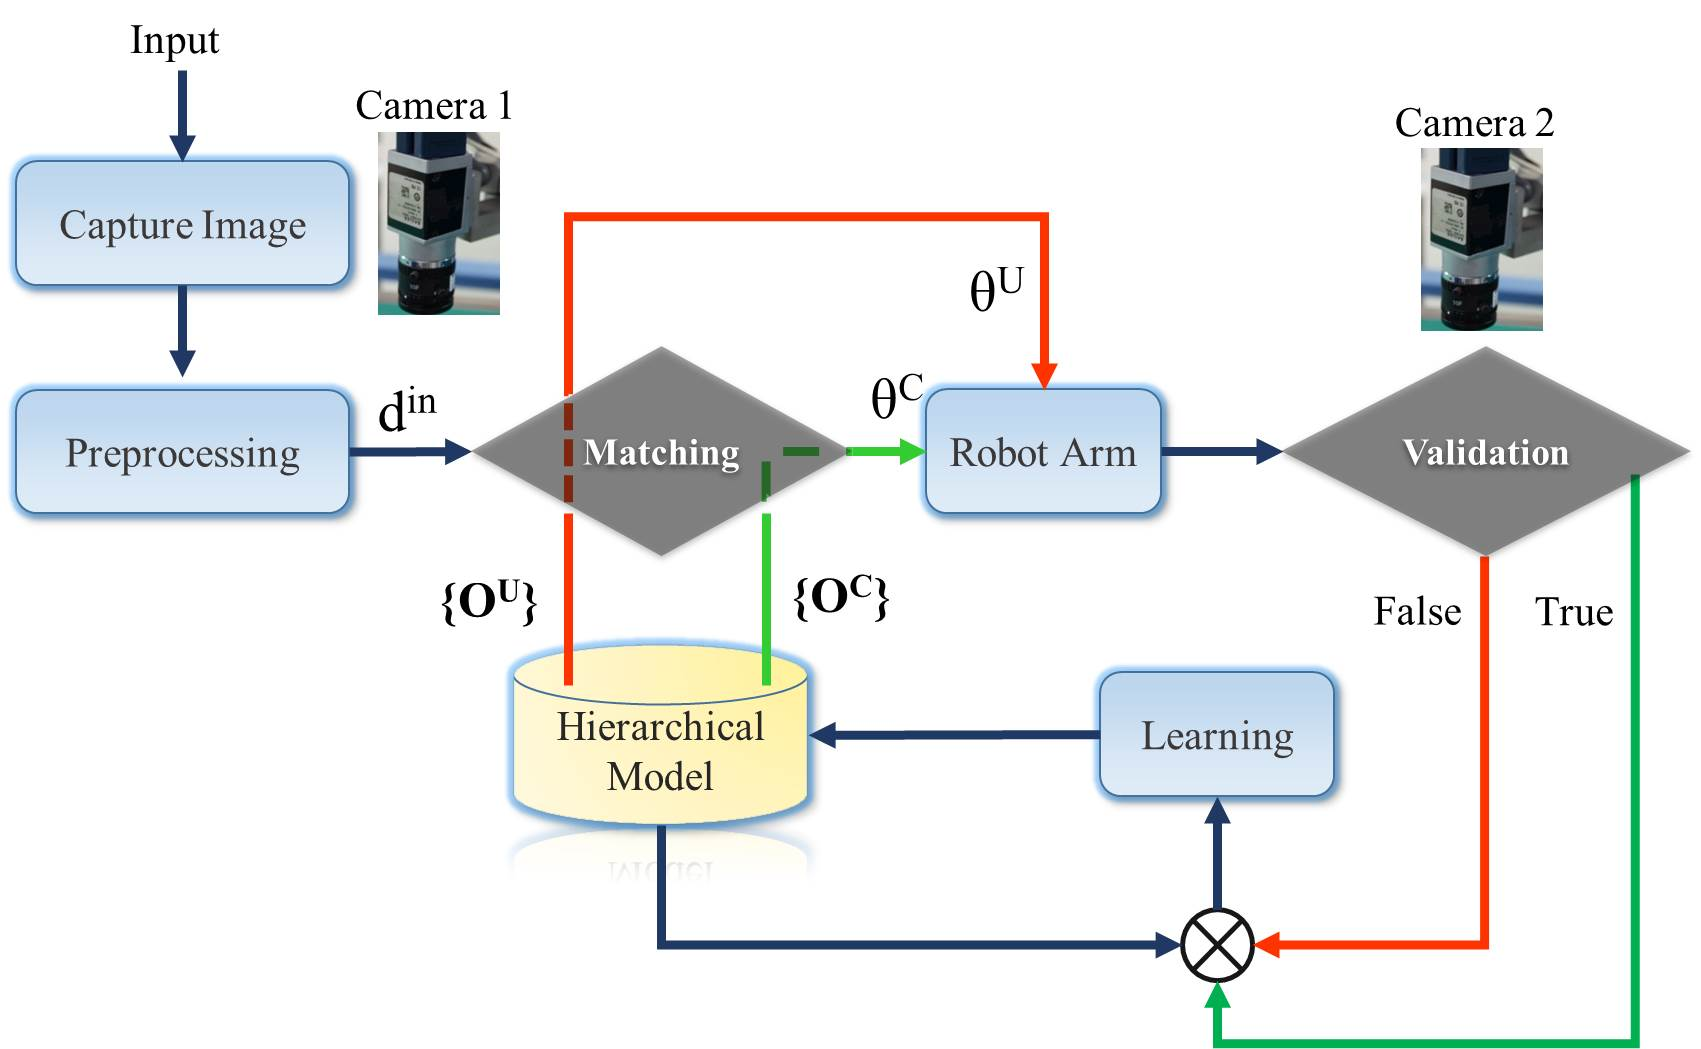
\includegraphics[width=0.5\textwidth]{j_img/fig1.jpg}
\caption{System architecture}\label{test}
\end{center}
\end{figure}

\begin{figure*}[!t]
\begin{center}
\includegraphics*[width=7 in]{j_img/fig3.jpg}
\caption{Hierarchical-deep model for self-taught system}\label{test}
\end{center}
\end{figure*}


%\hfill mds
\section{System architecture} 

The main purpose of this system is to automatically derive the relationship between input face and corresponding rotation angle to make robot arm can rotate objects to the assigned faces. The only prior knowledge are the target face. Input is arbitrary assigned object with random face on top, so input is very likely an unknown face of assigned object showed-up rather than prior target face. Therefore, system has to infer the correlation between input and existed priors.  Proposed system is shown in Fig. 1. Camera 1 captures images of all input objects with random faces on top, and constructs MLN-based descriptor for each input. Then, system matches the input with data in database and output rotation angle for robot arm. After robot arm placing an object, camera 2 will validate result, and feedback error for refining existed model. The system architecture in Fig. 1 is realized by a hierarchical-deep model in Fig. 2. 

The variables in the same layer are independent, and vertical adjacent two layers are full connected. Variables in \textbf{Feature($\bf{\Gamma}$)} layer are extracted image features, and variables in both \textbf{Classified Descriptor($\bf{D^C}$)} and \textbf{Unclassified Descriptor($\bf{D^U}$)} are MLN-based descriptor. Variables in \textbf{Rotation angle($\bf{\Theta^{C}}$)} and \textbf{Inferred Rotation angle($\bf{\Theta^U}$)} are set of rotation angles $\{$ Row ($\alpha$), Pitch($\beta$) , Yaw($\gamma$) $\}$ respect to target faces. Finally, variables in \textbf{Object($\bf{O^C}$)} are combinations of rotation angles.


The difference between classic \textbf{Deep Belief Networks}(\textbf{DBN}) is that proposed model exist two parallel parts in Fig. 2. \textbf{$\bf{D^C}$-$\bf{\Theta^{C}}$} and \textbf{$\bf{D^U}$-$\bf{\Theta^U}$} have no connection between each other, but both have full connection with deepest layer $\bf{O^C}$ and first layer \textbf{$\bf\Gamma$}. To handle tons of unknown data, the structure of connection will dynamically change with observed evidences. Sparse coding method is used to constructs edge in the model, most of connection is zero which is called latent edge in this paper. Latent edge might become non-zero while some new evidences have been discovered. For variable $d^C_w$ in layer $\bf{D^C}$, the sparse coding result should be formulated as:

\begin{equation}
d^C_w=\sum_{i\in{d^C_w}}a_{i}\Gamma_{i}+\sum_{j\notin{d^C_w}}b_{j}\Gamma_{j}
\end{equation}

Although Eq.(1) can handle the problem of latent edge, it's impractical to sample all possible conditions whenever new evidence showing up. Therefore, proposed model separate descriptor layer into two parallel parts as: 

\begin{equation}
d^C_w=\sum_{\Gamma_{i}\in{d^C_w}}a_{i}\Gamma_{i}
\end{equation}
\begin{equation}
d^U_r=\sum_{\Gamma_{j}\in{d^U_r}}b_{j}\Gamma_{j}
\end{equation}

$d^C_w$ is a prior descriptor which the edge between $\bf{\Theta^{C}}$ and $\bf{O^C}$ had been established. $d^U_r$ is a descriptor in $\bf{D^U}$ layer which match none of descriptors in $\bf{D^C}$. Therefore, we propose an inference method to infer the possible rotation angle, and camera 2 will check inferred results. If inference is success, latent edge between $d^U_r$ and $\theta^{U}$ will be established, and become stronger as more successful inferences.

\begin{figure}[!t]
\begin{center}
\subfigure[Result of background subtracton and clustering]{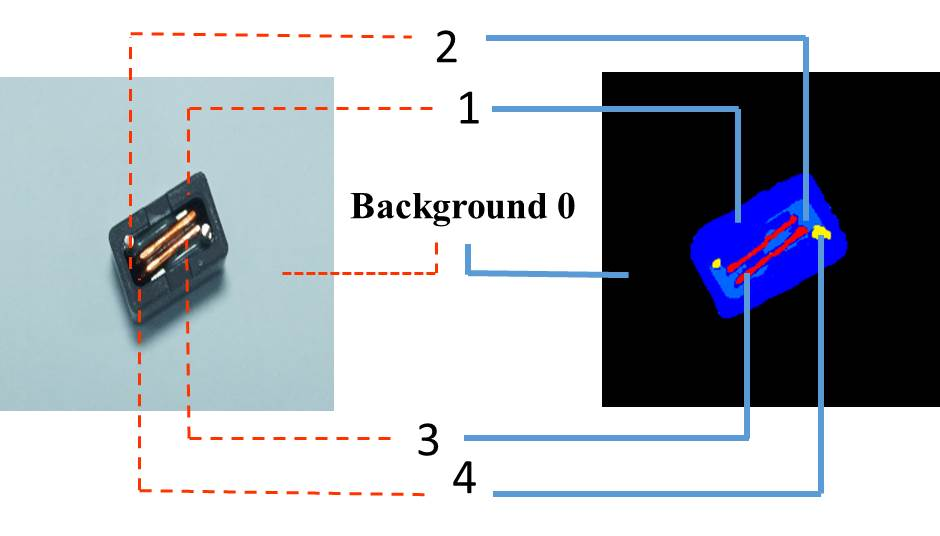
\includegraphics[width=3in]{j_img/fig2b.jpg}}
\subfigure[Serial captured frames]{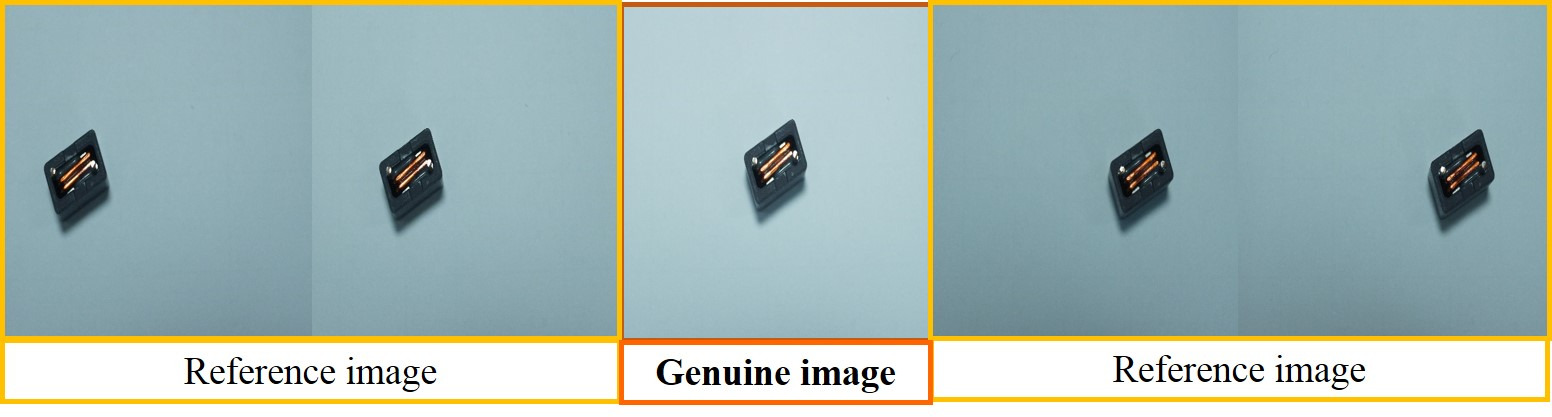
\includegraphics[width=3.5in]{j_img/fig2a.jpg}}
\caption{Preprocessing of input objects}\label{test}
\end{center}
\end{figure}


\section{MLN-based Descriptor}
\subsection{The concept of constructing MLN-based descriptor}
Being a self-taught system, deriving more valuable information from raw data helps system deriving more reliable results with scarce prior knowledge. Most of present image descriptors [12-16] are constructed based on strong sparse feature point, because these points are consistent even in different environment. These kinds of descriptor can efficiently and precisely match given image. Nevertheless, most of observed face is not in prior data, so we need a descriptor which can infer the relation between observations and priors. To avoid losing information, we choose normal distributed feature instead of sparse feature. Since different faces of an object may derive different strong features, normal distributed feature is more suitable for our case. 

For prepossessing of input images, each channel of RGB domain is classified into 5 parts, and get 125 classes in RGB domain. Every input image is segmented by these classes. In Fig. 3(a), an observed face of input object is segmented into 4 classes, and class 0 is background. Hereafter, predicates for MLN networks are constructed by segmented results. We have only two kinds of predicate \textit{ne(a,v)} and  \textit{des(x)} for MLN model. Variable \textit{a} is an atom cluster, and variable \textit{v} is a neighbor of atom cluster, so predicate \textit{ne(a,v)} represent adjacency of atom cluster. Variable \textit{x} in \textit{des(x)} is a MLN-based descriptor. The variables of \textbf{$\bf\Gamma$} layer in Fig. 2 are predicates \textit{ne(a,v)}. Since every class can be the atom cluster, we have $\binom{125}{2}$ binary variables in \textbf{$\bf\Gamma$} layer.

Taking Fig. 3(a) as an example, the predicates of preprocessed image are shown in Table \uppercase\expandafter{\romannumeral1}, and first order logic is formulated as:

\begin{equation}
\forall{a}\forall{v}\quad\textit{ne(a,v)}\Rightarrow\textit{des(x)}
\end{equation}

Each image will further be down sampled, and derived several images with different scales. For each image, we derive  \textbf{F*S} formulas where F is number of serial captured images and S is number of images with different scales. Through these formulas, a MLN model can be constructed. The probability distribution over possible world $d^{in}$ specified by MLN is given by:

\begin{displaymath}
P(\bf{D^{in}} = d^{in}) = \frac{1}{Z}exp(\sum_{j=1}^{F*S} w_j n_j(d^{in}))
\end{displaymath}
\begin{equation}
\bf{Z}=\sum_{d^{in}\in\bf{D^{in}}}exp(\sum_{j=1}^{F*S} w_j n_j(d^{in}))
\end{equation}

Where $d^{in}$ is the descriptor of input image. $n_j(d^{in})$ is the number of true grounding of formula j in $d^{in}$, and $w_j$ is weight of formula j .

Consequently, probability distribution Eq.(5) is MLN-based descriptor for each 2D faces within input 3D object. 

\begin{table}[!t]
\caption{Example of predicates}
\centering
\begin{tabular}{|c|c|c|c|c|} 
\hline
Key Atom & 1 & 2 & 3 & 4\\
\hline\hline
\multirow{4}{*}{Predicates} & 
ne(1,2) & 
ne(2,1) & 
ne(3,1) &
ne(4,1)\\
\cline{2-5}
 &
ne(1,3) &
ne(2,3) &
ne(3,2) &
ne(4,2) \\
\cline{2-5}
 &
ne(1,4) &
ne(2,4) &
 &
 \\
\cline{2-5}
 &
ne(1,0) &
 &
 &
 \\
\hline
\end{tabular} 
\end{table} 





\subsection{Inference and Weight learning of MLN-based descriptor}
The weights of MLN-based descriptor are learned by maximizing the pseudo-log likelihood. Since each descriptor can be consider as a closed world, we only need to consider the atoms which derive from captured serial frames. Comparing with uniform sampling approach, maximizing pseudo-log-likelihood is more efficient, because pseudo-log likelihood only need to consider relational data. The pseudo-log likelihood of Eq.(5) can be written as:

\begin{equation}
\log P^*_w(\mathbf{D^{in}} = d^{in}) = \sum_{j=1}^{F*S} \log P_{w}(\mathbf{D^{in}} = d^{in}|\mathbf{MB}(d^{in}))
\end{equation}

Where $\bf{MB}(d^{in})$ is Markov blanket while $d^{in}$ is observed. The MLN weights are learned generatively by maximizing the pseudo-log likelihood of Markov blanket. The gradient of the pseudo-log likelihood with respect to the weight is:

\begin{displaymath}
\begin{array}{ll}
\dfrac{\partial}{\partial w_i}\log P^*_w(\mathbf{D^{in}} = d^{in})= &\\\\
\sum^{F*S}_{j=1}\{n_i(d^{in})-P_w(\mathbf{D^{in}}=0|\mathbf{MB}(d^{in}))n_i(d^{in}=0) &\\
\end{array}
\end{displaymath}
\begin{equation}
-P_w(\mathbf{D^{in}}=1|\mathbf{MB}(d^{in})n_i(d^{in}=1)\}
\end{equation}

Where $n_i(d^{in}=0)$ is the number of true grounding of $j^{th}$ formula while force $\mathbf{d^{in}}=0$, and similar for $n_i(d^{in}=1)$. The learning of pseudo-log-likelihood in our approach are further boosted by  \textbf{\textit{Limited-memory Broyden-Fletcher-Goldfarb-Shanno(L-BFGS)}} optimizer [20] to make entire process become more efficiency.

\subsection{Matching of MLN-based descriptors}
For each constructed input descriptor $d^{in}_k$, system would search for the matched descriptor in the database, and further arrange it to the proper layer of $\bf{D^C}$ or $\bf{D^U}$ as shown in Fig.2. Since input is possible to be assigned to one of parallel layers, matching step is separated into two parts. One is using pseudo-log likelihood for deciding observation should be assigned to which layer. The pseudo-log likelihood of descriptors matching could be formulated as:


\begin{equation}
\begin{array}{ll}

\mathbf{argMax}P(\mathbf{D^C} = d^C_w  | \mathbf{D^{in}} = d^{in} , \mathbf{\Gamma}_{k \in {d^{in}}}) &\\\\
= \mathbf{argMax}P(d^{in} | \mathbf{MB}(d^{in}){P(d^{C}_w | \mathbf{MB}(d^{in}))}
\end{array}
\end{equation}


If input descriptors match none of descriptor in $\bf{D^C}$ layer, the descriptor become a variable of  $\bf{D^U}$ layer. For a variable in $\bf{D^U}$, we infer rotation angle to make input object which can be placed on corresponding target face. Since the rotation angles for descriptors in $\bf{D^U}$ are unidentified, the second part for matching is trying to find a descriptor in $\bf{D^C}$ which have max co-cluster with input descriptor. Finding max co-cluster can be alternately considered as minimizing information loss as:
\begin{equation}
\mathbf{argMin}(I(d^in , \mathbf{\Gamma}_{k \in d^{in} \cap d^C_w}) - I(d^C_w , \mathbf{\Gamma}_{k \in d^{in} \cap d^C_w}))
\end{equation}

The common feature $\mathbf{\Gamma}_{k \in d^{in} \cap d^C_w}$ is further represented by Markov Blanket of $d^{in}$ and $d^C_w$, and the loss of mutual information can be further formulated by \textbf{\textit{Kullback–Leibler divergence(KL divergence)}}[28] as:

\begin{equation}
\begin{array}{ll}
\mathbf{argMin}D(P(d^{in} , \mathbf{MB}(d^{in},d^c_w))||P(d^c_w , \mathbf{MB}(d^{in},d^c_w)))\\\\
= \mathbf{argMin}\sum_{\Gamma_k\in\mathbf{MB}(d^{in},d^c_w)}P(\Gamma_k)D(P(d^{in}|\Gamma_k)||P(d^C_w|\Gamma_k))\\\\
\end{array}
\end{equation}

In Eq.(10), classified descriptor $d^C_w$ with min KL divergence is considered as acquired max co-cluster with $d^{in}$. The relation between the co-cluster become the evidence for inferring rotation angle of $d^{in}$. Through Eq.(8) and Eq.(10), the input descriptors are classified to corresponding layer, and become inputs $\bf{\Theta^{U}}$ or $\bf{\Theta^{C}}$ layer.


\section{Hierarchical model}
\subsection{Inference of rotation angle in $\bf{\Theta^{U}}$ layer}
Inference rotation angle $\bf{\theta^{U}_i}$ is based on max co-cluster between $d^{in}$ and $d^C_w$. A set of co-cluster $\{$$C_{w1}$, $C_{w2}$, ..., $C_{wL}$$\}$ can be derived by minimizing KL divergence. The center of co-cluster with respect to center of camera in Cartesian space can be derived into two sets $\bf{V^{in}}$=$\{$$v^{in}_1$, $v^{in}_2$, ..., $v^{in}_L$ $\}$ and $\bf{V^{C}_w}$=$\{$$v^{C}_{w1}$, $v^{C}_{w2}$, ..., $v^{C}_{wL}$ $\}$. $\bf{V^{in}}$ is a set of co-cluster position in input descriptor, and $\bf{V^{C}_w}$ is a set of co-cluster position in $d^C_w$. The roll angle $\alpha$ of robot arm is calculated by:

\begin{equation}
\alpha =\cos^{-1}\frac{1}{L}\sum_{l=1}^K\frac{v^C_{wl}-v^{in}_l}{|v^C_{wl}-v^{in}_l|}
\end{equation}

Where roll angle $\alpha$ is the mean angle of co-cluster in two descriptors. As for  pitch angle $\beta$ and yaw angle $\gamma$, the pitch and yaw angle are hard to be estimated by 2D descriptor directly. We make random sample these two angles in value $\pi/2$ , and $-\pi/2$ initially, and approximate to actual angles by algorithm 1.



\begin{algorithm}
  \caption{Inferring rotation angle from co-cluster}
   $\bf{Function}$ inferringTheta$(d^{in},\bf{D^C},\bf{D^U})$\\ 
  $\bf{Input:}$\\
   $d^{in}$, input descriptor\\
   $\bf{D^C}$, descriptors in $\bf{D^C}$ layer\\
   $\bf{D^U}$, descriptors in $\bf{D^U}$ layer\\
  $\bf{Output:}$\\
  $\theta^U\{\alpha,\beta,\gamma\}$, rotation angle for robot arm\\        
  \begin{algorithmic}[1]
    \State $L\_{D^c} \leftarrow$ maxLikelihood($d^{in}$, $\bf{D^C}$)
    \State $L\_{D^U} \leftarrow$ maxLikelihood($d^{in}$, $\bf{D^U}$)
    \If{$L\_{D^U} > L\_{D^U}$}
    
 	$d\_target \leftarrow $ maxLikelihood($d^{in}$, $\bf{MB}$ in $\bf{D^U}$)
 		
 	$\theta^U\leftarrow$findmax$\_$Coclass($d^{in}$, $d\_target$)
 	
 		\While{t $<$ max$\_$t $||$ maxLikelihood(t)$>$ threshold}
 		
 			\If{maxLikelihood(t) $>$ maxLikelihood(t-1)}
 			
 				$\;\;\;\;\;\;t++$
 				
 				$\;\;\;\;\;\;\theta^U \leftarrow \theta^U+Step$
 				
 			\Else
 			
 				$\;\;\;\;\;\;Break$
 			\EndIf
 		
 		
 		
    	\EndWhile
    \Else
    
    	$d\_target \leftarrow $ maxLikelihood($d^{in}$, $\bf{MB}$ in $\bf{D^C}$)
    	
    	$\theta^U\leftarrow$findmax$\_$Coclass($d^{in}$, $d\_target$)
    \EndIf
    
	\State $\bf{Return}$ $\theta^U\{\alpha,\beta,\gamma\}$
    
  \end{algorithmic}
\end{algorithm}

\subsection{Inference and learning of hierarchical-deep model}

\begin{figure}[!t]
\begin{center}
\includegraphics*[width=2.5 in]{j_img/fig4.jpg}
\caption{Structure configuration of each layer in the proposed model}\label{test}
\end{center}
\end{figure}

Proposed hierarchical model is a generative model of \textbf{\textit{Deep Belief Network (DBN)}}. Structure between each layer is shown in Fig. 4. each layer is considered as a \textbf{\textit{Restricted Boltzmann Machine (RBM)}}[8] except $\bf{\Gamma}$, $\bf{D^C}$, and $\bf{D^U}$. The MLN is trained by pseudo-log likelihood as mentioned previously, and RBM is trained by greedy layer-wise training [30].

Initially, left part of model ($\bf{\Gamma}$-$\bf{D^C}$-$\bf{\Theta^C}$-$\bf{O^C}$) are trained with prior target face of objects, and number of variables $\bf{N}$ in $\bf{O^C}$ equal to the number of prior target faces. The right part of model is activated only when a new observation is classified into $\bf{D^U}$. The activation probability of $\theta^U_i$ is a sigmoid activation function:

\begin{equation}
\begin{array}{ll}
P(\theta^U_i|\bf{MB}(d^{in}))=\frac{1}{1+exp \left( \mu*b-\sum_r d^U_r w_{r}\right)} \\\\
\mu = \left\{
        \begin{array}{ll}
         0  & ,\mbox{if inference succeed} \\
         1+logP(\theta^U_i|\bf{\Theta^U}) & ,\mbox{if inference fail} \\ 
		\end{array}
	   \right.
\end{array}
\end{equation}



where $w_r$ and $b$ are the weights and bias. $\mu$ is penalty factor which decreases the probability while the inference is failed. $\mu$ is depended on log likelihood of $\theta^U_i$ which can lead to lower activation probability if inference result failed several times, and avoid system derives wrong results over again. 
On the other hand, for both $\bf{\Theta^U}$ and $\bf{\Theta^C}$ layer, if results are correct, the model will be retrained by greedy layer-wise training. If validated result is derived from left part of Fig. 4, the generative model is defined by the joint distribution of top layers $P(\bf{O^C} , \bf{\Theta^C})$. If the result is derived from right part, the generative model is defined by  $P(\bf{O^C} , \bf{\Theta^U})$. By doing so, the relation between prior and observations can be self-taught from numerous random unlabeled inputs, and infer possible relationship without any manual interference.



\section{Experiments}
The experiments for proposed model are separated into two parts. Firstly, we evaluate the performance of MLN-based descriptor by standard object recognition datasets: $\bf{Caltech-101}$ [31] and $\bf{Caltech-256}$ [32]. Results shown in Table \uppercase\expandafter{\romannumeral2} are comparisons with recently published papers. The images in the datasets are rescaled into five different scales for training proposed MLN-based descriptor. For $\bf{Caltech-101}$, we follow general procedure and randomly selecting 30 images for each class. For $\bf{Caltech-256}$, select 45 and 60 images for each class, and trained by pseudo-log likelihood. Although, for the proposed model, the result does not outperform in $\bf{Caltech-101}$, but the accuracy in $\bf{Caltech-256}$ is slightly behind ImageNet-pretrained model. In the other scopes, the result shows that MLN-based descriptor keep well performance even increasing categories. Most of recently published methods get dramatically performance decreasing while categories increase from 101 to 256. 


\begin{table}[!t]
\caption{Comparisons on $\bf{Caltech-101}$}
\begin{center}
\begin{tabular}{|c|c|}
\hline
Methods & Accuracy \\
\hline
$\bf{MLN-based}$ & $\bf{74.6}$ \\
\hline
LLC[37] & 73.1 \\
\hline
P-LLC[38] & 78.75\\
\hline
P-FV[38] & 80.1\\
\hline
M-HMP[39] & 82.5 \\
\hline
ImageNet-pretrained convnet[40] & 86.5 \\
\hline
\end{tabular}
\end{center}
\end{table}

\begin{table}[!t]
\caption{Comparisons on $\bf{Caltech-256}$}
\begin{center}
\begin{tabular}{|c|c|c|}
\hline
Methods & 45 & 60 \\
\hline
$\bf{MLN-based}$ & $\bf{66.7}$ & $\bf{69.6}$ \\
\hline
LLC &  45.3 & 47.7\\
\hline
P-LLC & 44.9 & 48.0\\
\hline
P-FV & 44.9 & 52.6\\
\hline
M-HMP & 54.8 & 58 \\
\hline
ImageNet-pretrained convnet & 72.7 & 74.2 \\
\hline
\end{tabular}
\end{center}
\end{table}



\begin{table*}[!t]
\caption{Three classes of testing work pieces for experiments}
\begin{center}
\begin{tabular}{|c|c||c|c||c|c|}
\hline
\multicolumn{2}{|c||}{\bf{WP1}} & \multicolumn{2}{c||}{\bf{WP2}} & \multicolumn{2}{c|}{\bf{WP3}}\\
\hline\hline
WP1.1 & WP1.5 & WP 2.1 & WP 2.5 & WP3.1 & WP3.5\\
\hline
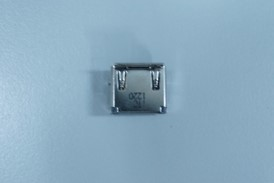
\includegraphics[width=1in,height=0.6in]{j_img/wp11.jpg} & 
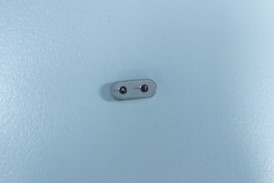
\includegraphics[width=1in,height=0.6in]{j_img/wp15.jpg} & 
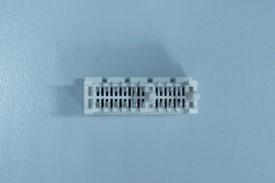
\includegraphics[width=1in,height=0.6in]{j_img/wp21.jpg} & 
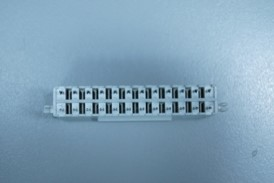
\includegraphics[width=1in,height=0.6in]{j_img/wp25.jpg} &
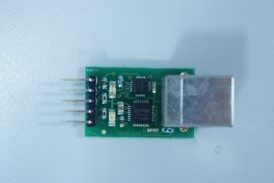
\includegraphics[width=1in,height=0.6in]{j_img/wp31.jpg} & 
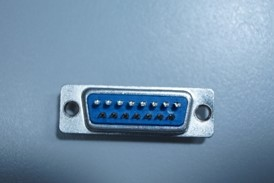
\includegraphics[width=1in,height=0.6in]{j_img/wp35.jpg} \\
\hline
WP1.2 & WP1.6 & WP 2.2 & WP 2.6 & WP3.2 & WP3.6\\
\hline
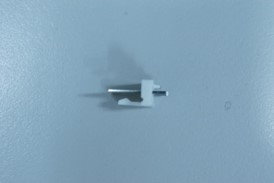
\includegraphics[width=1in,height=0.6in]{j_img/wp12.jpg} & 
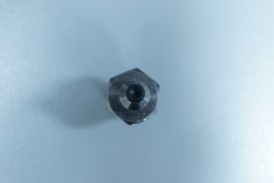
\includegraphics[width=1in,height=0.6in]{j_img/wp16.jpg} & 
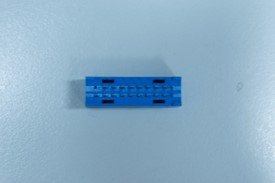
\includegraphics[width=1in,height=0.6in]{j_img/wp22.jpg} & 
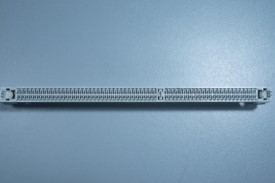
\includegraphics[width=1in,height=0.6in]{j_img/wp26.jpg} &
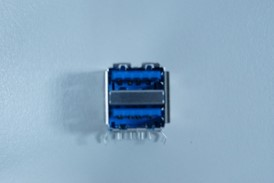
\includegraphics[width=1in,height=0.6in]{j_img/wp32.jpg} & 
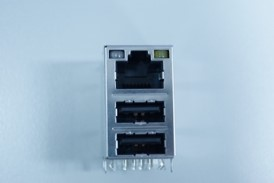
\includegraphics[width=1in,height=0.6in]{j_img/wp36.jpg} 
\\
\hline
WP1.3 & WP1.7 & WP 2.3 & & WP3.3 & WP3.7\\
\hline
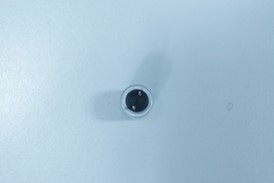
\includegraphics[width=1in,height=0.6in]{j_img/wp13.jpg} & 
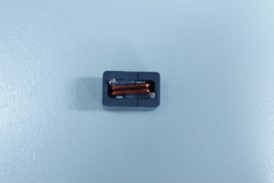
\includegraphics[width=1in,height=0.6in]{j_img/wp17.jpg} & 
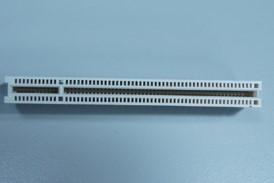
\includegraphics[width=1in,height=0.6in]{j_img/wp23.jpg} & 
 &
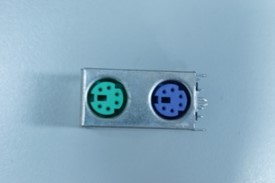
\includegraphics[width=1in,height=0.6in]{j_img/wp33.jpg} & 
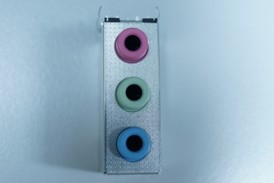
\includegraphics[width=1in,height=0.6in]{j_img/wp37.jpg} 
\\
\hline
WP1.4 & & WP 2.4 & & WP3.4 &\\
\hline
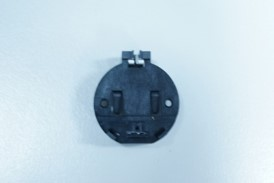
\includegraphics[width=1in,height=0.6in]{j_img/wp14.jpg} & 
 & 
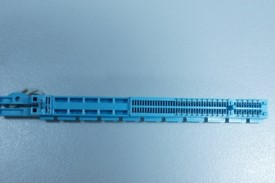
\includegraphics[width=1in,height=0.6in]{j_img/wp24.jpg} & 
 &
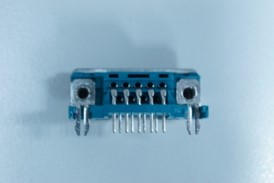
\includegraphics[width=1in,height=0.6in]{j_img/wp34.jpg} & 
\\ 
\hline
\end{tabular}
\end{center}
\end{table*}

For the second part of experiment, we implement the proposed system in real industrial application. The prior knowledge is target faces of assigned objects, and there are twenty kinds of assigned objects in our experiment. Table \uppercase\expandafter{\romannumeral4} shows twenty target faces for each assigned object. The experiment is implemented based on several assumptions: The input objects are not occluded, and not adjacent with each other. Hereafter, the inputs are randomly chosen from assigned objects with random face on top. 

The testing objects are classified into three classes in Table \uppercase\expandafter{\romannumeral4}. For class $\bf{WP1}$, the work pieces are featureless and relative small, so it's hard to construct robustness descriptor even building relational model for entire model. For class $\bf{WP2}$, all work pieces acquire similar shapes and size, so this kind of object is easily mismatched in the matching process. The work pieces in $\bf{WP3}$ are matched group of this experiment. These work pieces acquire sufficient features for descriptor, and have plenty of information for identifying and constructing descriptor. In the first stage of experiment, we compare the performance of proposed system between different classes in different lighting conditions.  The results of different classes are shown in Fig.5. In Fig.5(a), the environment lighting is controlled by on-axis lighting source, so the information of object are more complete and distinct than images without lighting control in Fig.5(b). The accuracy is average of 100 times repeatedly testing.

The system is considered convergence while accuracy is over 95$\%$, and stop learning approach. If the accuracy is under 95$\%$ again, the learning approach would be re-excuted. Comparing the results, in both cases, class $\bf{WP3}$ could be convergent with least input sample, and convergent time of class $\bf{WP2}$ is slowest. The results show that the efficiency of learning could be slightly improved by environment constrain, but the accuracy is not effected, and always keep over 95$\%$ after learning approach stopped. 
 
Fig. 6 shows the result while all twenty kinds of assigned object are involved in the same time. The result shows that system need more inputs to converge while more kinds of objects are involved, but the system still slightly converge, and accuracy is all keeping over 95$\%$ for both conditions. In brief, these two experiments verify proposed system is competent to learn the HD model automatically. Although the learning rate is dragged by the number of assigned objects, the learning rate still can be convergent by reasonable number of inputs. 


 
\begin{figure}[!t]
\centering
	\subfigure[Performance with on-axis lighting source]{
		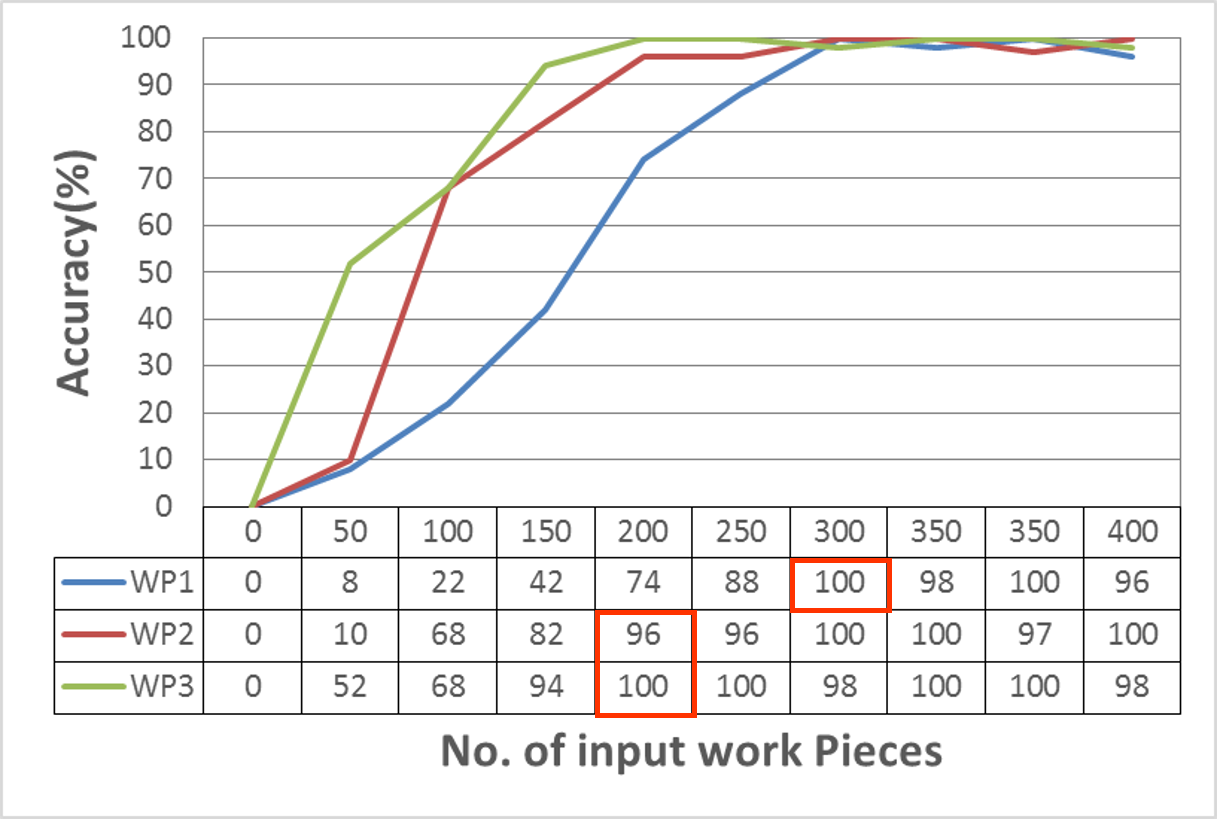
\includegraphics[width=3 in]{j_img/exp01.png}
	}

	\subfigure[Performance without on-axis lighting source]{
		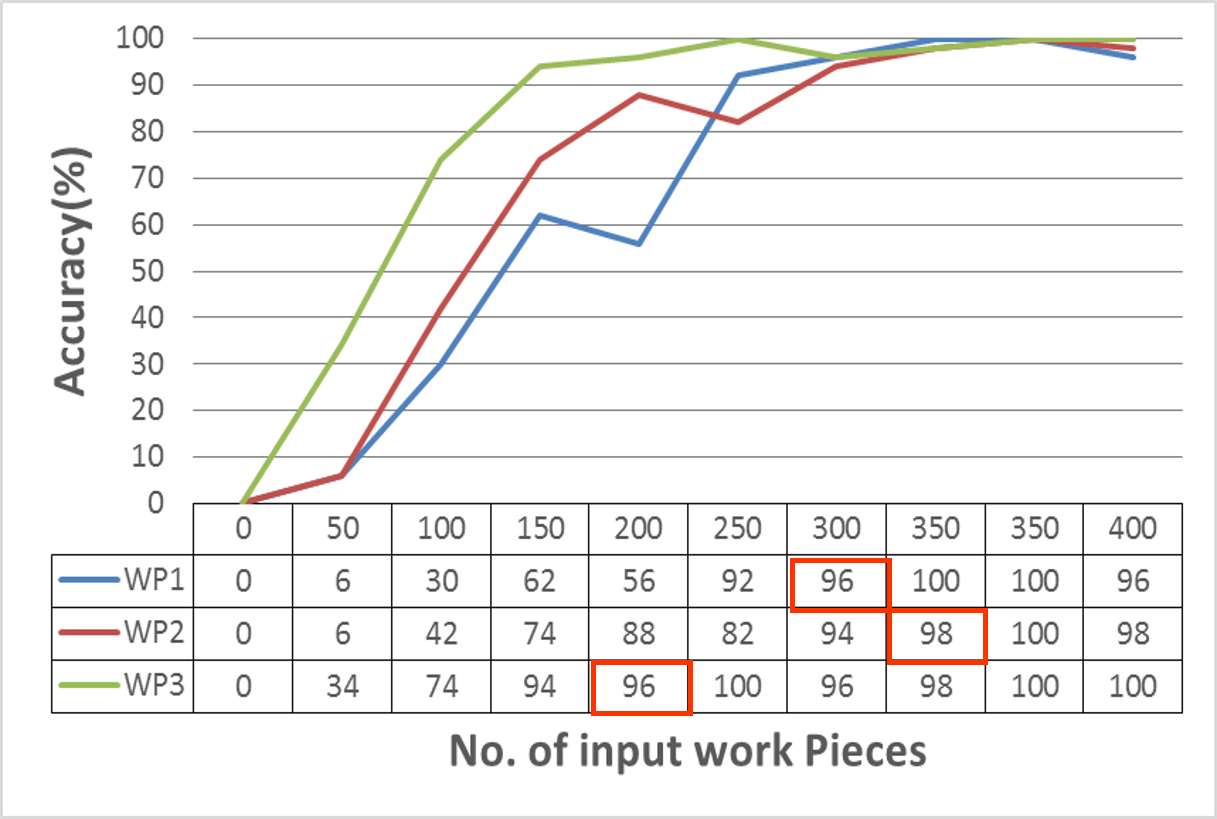
\includegraphics[width=3 in]{j_img/exp02.png}
	}

\caption{Experimental Results of different classes in different lighting conditions}

\end{figure}

\begin{figure}[!t]
\centering
	\subfigure[Performance with on-axis lighting source]{
		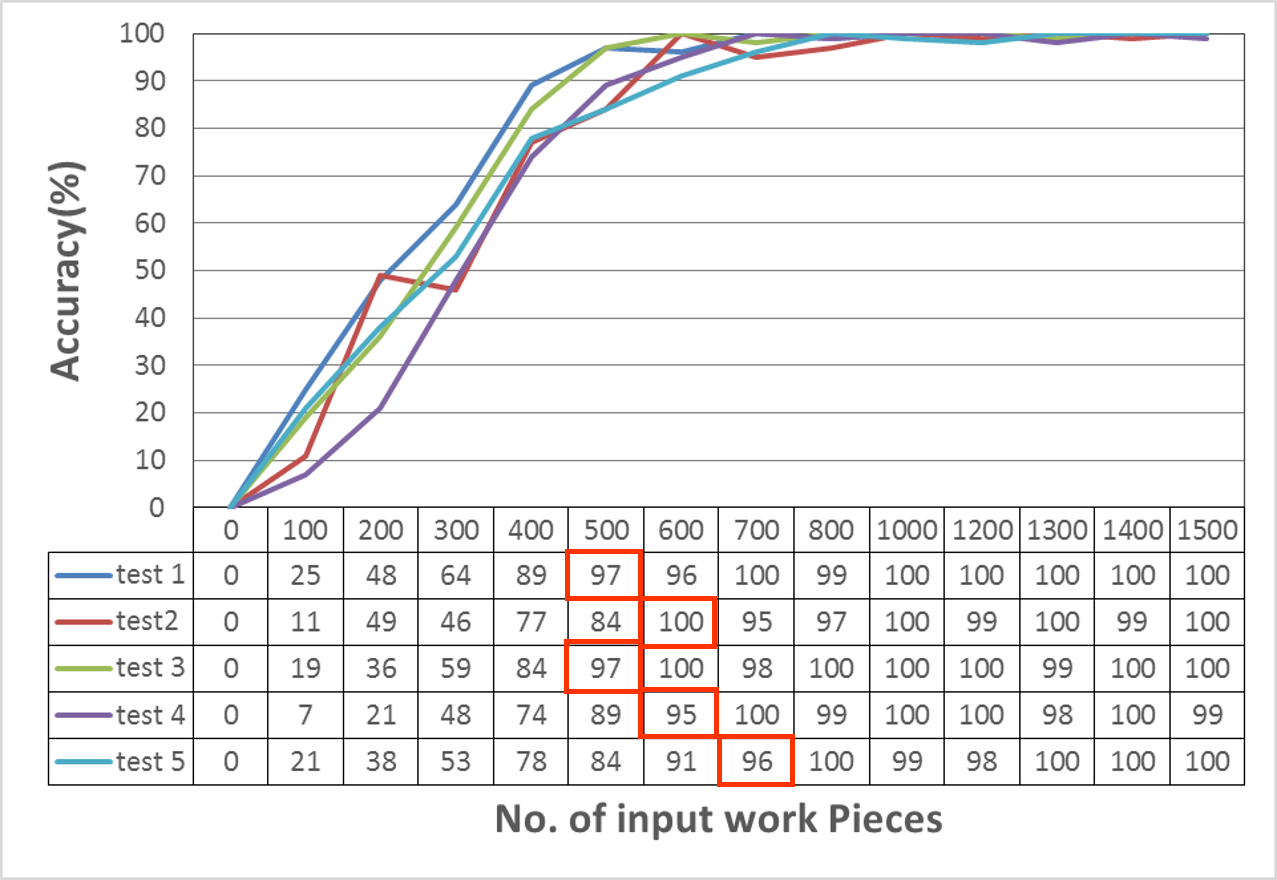
\includegraphics[width=3 in]{j_img/exp03.png}
	}

	\subfigure[Performance without on-axis lighting source]{
		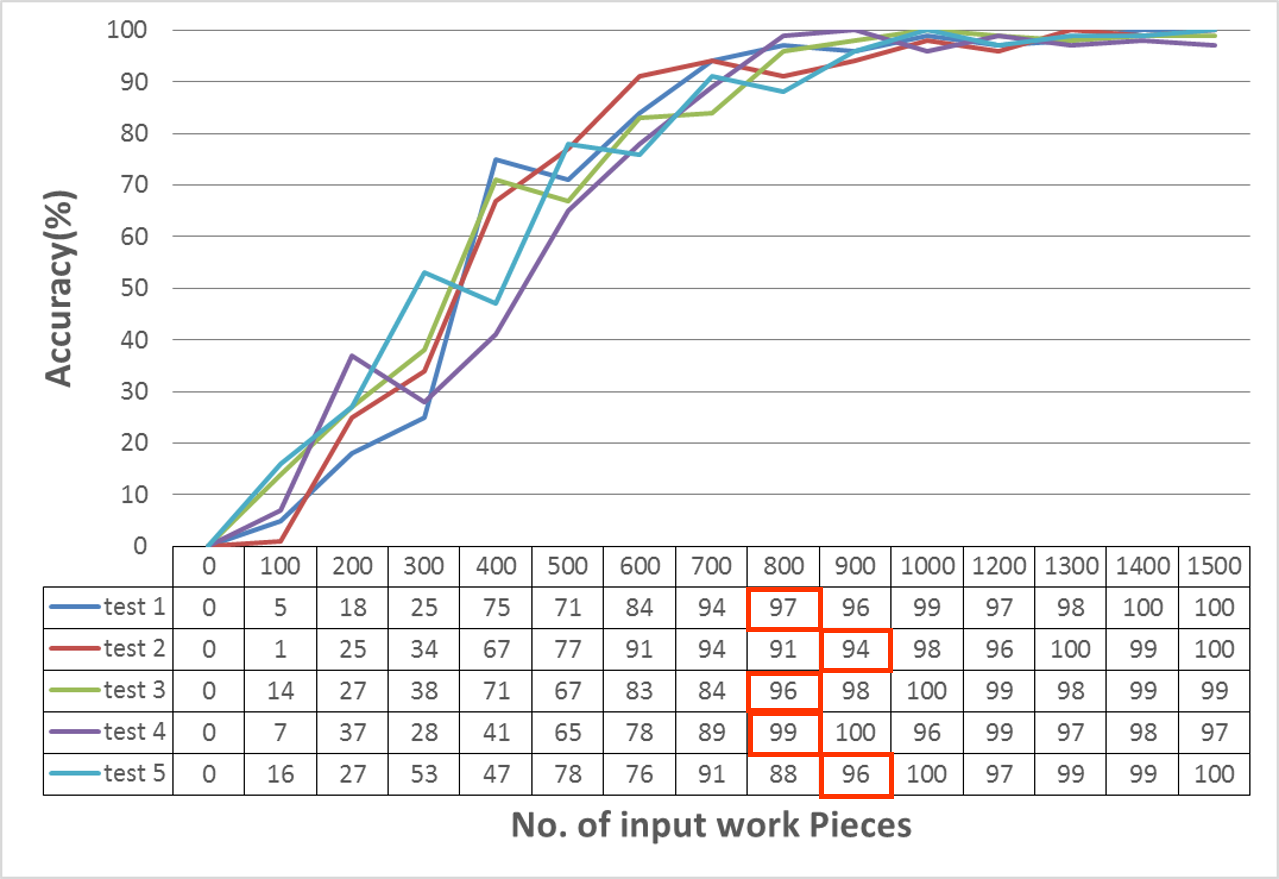
\includegraphics[width=3 in]{j_img/exp04.png}
	}

\caption{Experimental Results of all work pieces in different lighting conditions}

\end{figure}

The experiment in Fig. 5 and 6 testified the performance of proposed system can meet our requirements. We compare the performance of proposed system with other advanced approaches. Since none of similar systems could handle this issue in our literature survey results, so the comparisons are done by dividing our system into two parts. One is 2D descriptors for each face of objects, and the other is machine learning approach for learning relational model.

For the descriptor part, four kinds of other descriptors are chosen to compare with proposed system. B-SIFT[35]and Edge-SIFT[36] are modified versions of SIFT approach which enhanced the accuracy of feature point registration.  \textbf{\textit{Binary Robust Invariant Scalable Keypoints(BRISK)}}[15] descriptor is constructed based on binary robust invariant scalable key points, and \textbf{\textit{Zernike Moment (ZM)}}[13] phase-based descriptor is a moment-based descriptor which use the phase information of signal. All of these descriptors are representative methods in relative field recent years, and had been testified by many researchers. To compare the robustness and accuracy, the performance is testified by two conditions as shown in Table \uppercase\expandafter{\romannumeral5}. One is relationship of each face is prior of system, and the descriptors only provide information for object matching. The experiments are implemented by the same learning approach which is proposed in the previous section. The other is no prior for learning approach that information of descriptor need to be used for inferring the relational model. The ZM descriptor has the best performance in the condition with prior, but results of descriptors are close. In condition, without prior, the MLN-based descriptor acquires best performance which testified MLN-based descriptor is suited for handling large amount of unlabeled data. 

Hereafter, the performances of different learning methods are further discussed. The other three kinds of transfer learning approaches: \textbf{\textit{Locally Weighted Ensemble approach(LWE)}}[25], \textbf{\textit{Transductive SVM(TSVM)}}[26], and self-taught learning[21] are chosen to compare with proposed method. Similarly, the experiments are divided into two parts as shown in Table \uppercase\expandafter{\romannumeral6}. The result shows LEW acquires the best accuracy in the condition with priors, and proposed learning approach acquire greatest performance in condition without prior. Although the performances between different methods are quite close when priors are provided, the accuracy of the other methods goes down in no prior condition. It seems that the results are not only affected by descriptor, but also learning approach. The proposed system is only one method which can automatically learn and recognize object without prior knowledge of 3D model. 

\newcommand{\tabincell}[2]{\begin{tabular}{@{}#1@{}}#2\end{tabular}}

\begin{table}[!t]
\caption{Comparisons of different descriptors}
\centering
\begin{tabular}{|c|c|c|c|c|c|c|} 
\hline
\multirow{2}{*}{} &
&
\multicolumn{5}{|c|}{\bf{Descriptor}} \\
\cline{3-7}
 &
 & 
\bf{\tabincell{l}{MLN-\\based}} &
\bf{B-SIFT} &
\bf{\tabincell{l}{Edge-\\SIFT}} &
\bf{BRISK} &
\bf{ZM} 
 \\
\hline
\multirow{4}{*}{\tabincell{l}{With\\prior}} &
WP1 &
0.9781&
0.9664&
0.8384&
0.9556&
0.9788
\\
\cline{2-7}
&
WP2 &
0.9630&
0.9766&
0.9233&
0.9676&
0.9523
\\
\cline{2-7}
&
WP3 &
0.9901&
0.9963&
0.9454&
0.9899&
0.9949
\\
\cline{2-7}
&
All &
0.9594&
0.8982&
0.8066&
0.9432&
0.9634
\\
\hline\hline
\multirow{4}{*}{\tabincell{l}{Without\\prior}} &
WP1 &
0.9611&
0.7688&
0.7544&
0.8103&
0.7787
\\
\cline{2-7}
&
WP2 &
0.9505&
0.7043&
0.7123&
0.7197&
0.7979
\\
\cline{2-7}
&
WP3 &
0.9718&
0.8044&
0.7963&
0.8243&
0.8231
\\
\cline{2-7}
&
All &
0.9543&
0.6431&
0.6144&
0.6741&
0.7570
\\
\hline

\end{tabular} 
\end{table} 

\begin{table}[!t]
\caption{Comparisons of different learning approaches}
\centering
\begin{tabular}{|c|c|c|c|c|c|} 
\hline
\multirow{2}{*}{} &
&
\multicolumn{4}{|c|}{\bf{Learning approach}} \\
\cline{3-6}
 &
 & 
\bf{Proposed} &
\bf{LEW} &
\bf{TSVM} &
\bf{Self-taught} 
\\
\hline
\multirow{4}{*}{\tabincell{l}{With\\prior}} &
WP1 &
0.9781&
0.9802&
0.9511&
0.9603
\\
\cline{2-6}
&
WP2 &
0.9630&
0.9763&
0.9690&
0.9701
\\
\cline{2-6}
&
WP3 &
0.9901&
0.9899&
0.9799&
0.9807
\\
\cline{2-6}
&
All &
0.9594&
0.9677&
0.9567&
0.9701
\\
\hline\hline
\multirow{4}{*}{\tabincell{l}{Without\\prior}} &
WP1 &
0.9611&
0.5601&
0.6443&
0.6213

\\
\cline{2-6}
&
WP2 &
0.9505&
0.6543&
0.7158&
0.7128

\\
\cline{2-6}
&
WP3 &
0.9718&
0.7188&
0.7799&
0.7846

\\
\cline{2-6}
&
All &
0.9603&
0.6553&
0.7497&
0.7081
\\
\hline

\end{tabular} 
\end{table} 

\section{Comparisons of related works}
The proposed system is a HD model with parallel branches. Conventionally, the descriptors [13, 15, 35-39] and learning model [27-28] are separated, so the learning approaches only learn the distribution of descriptors but cannot adjust the distribution of descriptors. According to our surveys, no such a descriptor constructor can fit every case without manual interference. Therefore, the proposed approach takes an alternative way to make learning approach can adjust the distribution of descriptors to make the MLN-based descriptor can be refined during learning stage. This thought is proved by experimental results show in Table V and VI. The descriptors have to be constructed without manual interference in condition of without prior knowledge, and the result shows the performances of other than proposed method are dramatic decreased. 

Moreover, the other feature of proposed system is that learn knowledge in both image and rotation angle by just one model. Most of HD models [8-11] are focus on learning knowledge in the same domains, e.g.  handwriting [8], text categorization[9], Speech Recognition [10], images[11]. To handle the knowledge in different domains, we involve the technique of self-taught clustering and parallel structure model, and the experimental result also shows the feasibility of learning knowledge in different domains by proposed HD model.

\section{Conclusion}
An automatic learning system for vision system is an important part in assembling production line with small-volume, large-variety components. In this work, we reverse the concept of traditional vision system. The robustness of feature points and descriptor is not main concerns. Instead, the relation between input and output is the most essential. 

To learn the relationship between input and output, we propose a HD model which combines the concept of deep learning, transfer learning, and Markov logic network. The model acquires self-taught ability which can infer relational model and self-supervised the performance of learning results. Being an automatic system, tackling large amount of unlabeled data and inferring relation with labeled data is necessary. The relation between features in different levels can be represented as a discriminative distribution by the model. Through the discriminative distributions, KL divergence is further involved to find the max co-cluster between labeled and unlabeled data, and makes system stable under growing database. 

Moreover, proposed system includes image features, descriptors and rotation angles for robot arm. These different domain features are impossible to be learned simultaneously by traditional single layer model, but the experimental results prove proposed HD model can transfer and learn different domain knowledge, and recognize 3D object without manual interference. We believe this system is practical in real industrial assembling production line, and save labor cost.


 

.
\ifCLASSOPTIONcaptionsoff
  \newpage
\fi




\begin{thebibliography}{1}
%%%visual servo sta%%%
\bibitem{IEEEhowto:kopka}
Torgny Brogårdh, \emph{"Present and future robot control development—An industrial perspective"},\hskip 1em plus
  0.5em minus 0.4em\relax Annual Reviews in Control, Volume 31, Issue 1, pp. 69–79, 2007.

\bibitem{IEEEhowto:kopka} 
Ebrahim Mattar, \emph{"Robotics Arm Visual Servo: Estimation of Arm-Space Kinematics Relations with Epipolar Geometry, Robotic Systems - Applications, Control and Programming"},\hskip 1em plus
  0.5em minus 0.4em\relax Dr. Ashish Dutta (Ed.), ISBN: 978-953-307-941-7, InTech, DOI: 10.5772/25605.

\bibitem{IEEEhowto:kopka} 
So-Youn Park ,Yeoun-Jae Kim ,Ju-Jang Lee ,Byung Soo Kim, and Khalid A.Alsaif,\emph{"Controlling robot arm manipulator using image-based visual servoing without pre-depth information"},\hskip 1em plus 0.5em minus 0.4em\relax  37th IEEE Interantional Conferece on Industrial Electronics, pp.3157-3161,Nov. 2011.

\bibitem{IEEEhowto:kopka} 
K. Deguchi, H. Sakurai, and S. Ushida,\emph{"A Goal Oriented just-in-time visual servoing for ball catching robot arm”},\hskip 1em plus 0.5em minus 0.4em\relax in Int. Conf. on Intelligent Robots and Systems, Sept. 2008, pp. 3034–3039.
%%%visual servo end%%%

%%%single model sta%%%
\bibitem{IEEEhowto:kopka} 
J. Baker, L. Deng, J. Glass, S. Khudanpur, Chin hui Lee, N. Morgan, and D. O’Shaughnessy,\emph{" Developments and directions in speech
recognition and understanding, part 1"},\hskip 1em plus 0.5em minus 0.4em\relax Signal Processing Magazine, IEEE, vol. 26, no. 3, pp. 75–80, may 2009.

\bibitem{IEEEhowto:kopka} 
S. Furui,\emph{" Digital Speech Processing, Synthesis" },\hskip 1em plus 0.5em minus 0.4em\relax  Marcel Dekker, 2000.

\bibitem{IEEEhowto:kopka} 
Tong Simon, and Daphne Koller,\emph{"Support vector machine active learning with applications to text classification"},\hskip 1em plus 0.5em minus 0.4em\relax  The Journal of Machine Learning Research 2 pp 45-66, 2002.

%%%single model end%%%

%%%deep learning%%%

\bibitem{IEEEhowto:kopka} 
Hinton, G. E., Osindero, S. and Teh, Y,\emph{" A fast learning algorithm for deep belief nets" },\hskip 1em plus 0.5em minus 0.4em\relax Neural Computation, 18, pp 1527-1554,2006.
%%%deep learning%%%

%%%application of DL sta%%%

\bibitem{IEEEhowto:kopka} 
Srivastava, N., Salakhutdinov, R. R. and Hinton, G. E.,\emph{" Modeling Documents with a Deep Boltzmann Machine" },\hskip 1em plus 0.5em minus 0.4em\relax In IEEE International Conference on Acoustic Speech and Signal Processing (ICASSP 2013) Vancouver, 2013.

\bibitem{IEEEhowto:kopka} 
Graves, A., Mohamed, A. and Hinton, G. E,\emph{" Speech Recognition with Deep Recurrent Neural Networks" },\hskip 1em plus 0.5em minus 0.4em\relax In Uncertainty in Artificial Intelligence(UAI 2013).

\bibitem{IEEEhowto:kopka} 
Ranzato, M., Mnih, V., Susskind, J. and Hinton, G. E.,\emph{" Modeling Natural Images Using Gated MRFs" },\hskip 1em plus 0.5em minus 0.4em\relax IEEE Trans. Pattern Analysis and Machine Intelligence, 2013.
%%%application of DL end%%%

%%%2D image recognition sta%%%
\bibitem{IEEEhowto:kopka} 
H. Bay, A. Ess, T. Tuytelaars, and L. Gool,\emph{"SURF: Speeded up robust features"},\hskip 1em plus 0.5em minus 0.4em\relax Comput. Vis. Image Understand., vol. 110, no. 3, pp. 346–359, Mar. 2008.

\bibitem{IEEEhowto:kopka} 
Zen Chen and Shu-Kuo Sun,\emph{"A Zernike Moment Phase-Based Descriptor for Local
Image Representation and Matching"},\hskip 1em plus 0.5em minus 0.4em\relax IEEE Trans. Image
Process., vol. 19, no. 1,pp. 205–219, Jan. 2010.

\bibitem{IEEEhowto:kopka} 
A. Alahi, R. Ortiz, and P. Vandergheynst,\emph{"Freak: Fast retina keypoint"},\hskip 1em plus 0.5em minus 0.4em\relax CVPR, 2012.

\bibitem{IEEEhowto:kopka} 
S. Leutenegger, M. Chli, and R. Siegwart,\emph{"Brisk: Binary Robust Invariant Scalable Keypoints"},\hskip 1em plus 0.5em minus 0.4em\relax International conference on Computer Vision, 2011.

\bibitem{IEEEhowto:kopka} 
 Vijay Chandrasekhar, Gabriel Takacs, David Chen, Sam S. Tsai, Jatinder Singh, and Bernd Girod,\emph{"Transform coding of image feature descriptors,"},\hskip 1em plus 0.5em minus 0.4em\relax SPIE 7257, Visual Communications and Image Processing, 2009.

%%%2D image recognition sta%%%

%%%MLN sta%%%
\bibitem{IEEEhowto:kopka} 
Matthew Richardson and Pedro Domingos,\emph{"Markov logic networks,"},\hskip 1em plus 0.5em minus 0.4em\relax International Journal of Machine Learning, Volume 62, Issue 1-2,pp 107-136, Feb. 2006.

\bibitem{IEEEhowto:kopka} 
L. Mihalkova, T. Huynh, and R.J. Mooney,\emph{“Mapping and
Revising Markov Logic Networks for Transfer Learning”,},\hskip 1em plus 0.5em minus 0.4em\relax Proc. 22nd Assoc. for the Advancement of Artificial Intelligence (AAAI) Conf. Artificial Intelligence, pp 608-614, July 2007.

\bibitem{IEEEhowto:kopka} 
Kok, Stanley and Domingos, Pedro,\emph{"Learning the Structure of Markov Logic Networks"},\hskip 1em plus 0.5em minus 0.4em\relax Proceedings of the 22Nd International Conference on Machine Learning, pp 441-448, Germany, 2005.

\bibitem{IEEEhowto:kopka} 
Parag Singla and Pedro Domingos,\emph{"Discriminative training of Markov logic networks"},\hskip 1em plus 0.5em minus 0.4em\relax Proceedings of the international Conf. on Artificial Intelligence, 2005.
%%%MLN end%%%

%%%self-taught clustering sta%%%
\bibitem{IEEEhowto:kopka} 
Wenyuan Dai, Qiang Yang, Gui-Rong Xue and Yong Yu,\emph{"Self-taught Clustering"},\hskip 1em plus 0.5em minus 0.4em\relax Proceedings of the 25th International Conference on Machine Learning(ICML),2008.
%%%self-taught clustering end%%%

%%%transfer learning sta%%%

\bibitem{IEEEhowto:kopka} 
Sa\v{s}o D\v{z}eroski\emph{"Multi-relational Data Mining: An Introduction"},\hskip 1em plus 0.5em minus 0.4em\relax SIGKDD Explore Newsletter, Volume 5, Issue 1, July 2003, pp.1-16.


\bibitem{IEEEhowto:kopka} 
Sinno Jialin Pan, and  Qiang Yang,\emph{"A Survey on Transfer Learning"},\hskip 1em plus 0.5em minus 0.4em\relax Knowledge and Data Engineering, IEEE Transactions on , vol.22, no.10, pp.1345,1359, Oct. 2010


\bibitem{IEEEhowto:kopka} 
T. Dietterich, L. Getoor, and K. Murphy,\emph{"Statistical Relational Learning and its Connections to Other Fields"},\hskip 1em plus 0.5em minus 0.4em\relax ICML-2004 Workshop on Statistical Relational Learning (SRL), Banff, Canada, July 2004.


\bibitem{IEEEhowto:kopka} 
Jing Gao and Wei Fan and Jing Jiang and Jiawei Han, \emph{"Knowledge Transfer via Multiple Model Local Structure Mapping"},\hskip 1em plus 0.5em minus 0.4em\relax in the 14th ACM SIGKDD International Conference on Knowledge Discovery and Data Mining,pp. 283-291,New York, USA,2008

\bibitem{IEEEhowto:kopka} 
T. Joachims, \emph{"Making large-scale svm learning practical."},\hskip 1em plus 0.5em minus 0.4em\relax advances in kernel methods - support vector learning, MIT-Press, 1999.

\bibitem{IEEEhowto:kopka} 
A. J. Carlson, C. M. Cumby, J. L. R. Nicholas D. Rizzolo,
and D. Roth,\emph{"Snow learning architecture"},\hskip 1em plus 0.5em minus 0.4em\relax Technical report UIUCDCS, 1999.

%%%transfer learning end%%%

%%%DL divergence%%%%

\bibitem{IEEEhowto:kopka} 
Cover, T. M. and Thomas, J. A.,\emph{"Elements of
information theory"},\hskip 1em plus 0.5em minus 0.4em\relax Wiley-Interscience.
%%%DL divergence%%%%

%%%Greedy Layer-Wise Training%%%
\bibitem{IEEEhowto:kopka} 
Yoshua Bengio, Pascal Lamblin, Popovici Dan, and Larochelle Hugo,\emph{"Greedy Layer-Wise Training of Deep Networks"},\hskip 1em plus 0.5em minus 0.4em\relax Advances in Neural Information Processing Systems, 2007.
%%%Greedy Layer-Wise Training%%%

%%%Caltech 101 and 256%%%%

\bibitem{IEEEhowto:kopka} 
Fei-Fei Li, R. Fergus , and P. Perona ,\emph{" Learning generative visual models
from few training examples: an incremental Bayesian approach tested on
101 object categories"},\hskip 1em plus 0.5em minus 0.4em\relax IEEE. CVPR 2004, Workshop on Generative-Model Based Vision, 2004.

\bibitem{IEEEhowto:kopka} 
Griffin, G. Holub, and P. Perona ,\emph{" The Caltech 256"},\hskip 1em plus 0.5em minus 0.4em\relax Caltech Technical Report.

%%%Caltech 101 and 256%%%%

\bibitem{IEEEhowto:kopka} 
Karthikeyan Vaiapury, Anil  Aksay and Ebroul Izquierdo,\emph{"GrabcutD: Improved Grabcut Using Depth Information"},\hskip 1em plus 0.5em minus 0.4em\relax Proceedings of the 2010 ACM Workshop on Surreal Media and Virtual Cloning, pp 57-62, New York, USA, 2010.

\bibitem{IEEEhowto:kopka} 
Z. Zivkovic,\emph{"Improved adaptive Gaussian mixture model for background subtraction"},\hskip 1em plus 0.5em minus 0.4em\relax Pattern Recognition, 2004. ICPR 2004. Proceedings of the 17th International Conference on , vol.2, no., pp.28,31 Vol.2, 23-26 Aug. 2004.


\bibitem{IEEEhowto:kopka} 
Fei Sha and Fernando Pereira,\emph{"Shallow parsing with conditional
random fields"},\hskip 1em plus 0.5em minus 0.4em\relax Proceedings of the 2003 Conference of the North American Chapter of the Association for Computational Linguistics on Human Language Technology, Volume 1, 2003.

%%%Experiment sta%%%

\bibitem{IEEEhowto:kopka} 
Yanning Zhang,Zhi-Hua Zhou, Changshui Zhang and Li, Ying,\emph{"B-SIFT: A Highly Efficient Binary SIFT Descriptor for Invariant Feature Correspondence"},\hskip 1em plus 0.5em minus 0.4em\relax Intelligent Science and Intelligent Data Engineering, pp 426-433, 2012

\bibitem{IEEEhowto:kopka} 
S. Zhang, Q. Tian, K. Lu, Q. Huang and W. Gao,\emph{"Edge-SIFT: Discriminative binary descriptor for scalable partial-duplicate mobile search"},\hskip 1em plus 0.5em minus 0.4em\relax ” IEEE Trans. Image Process., vol. 22, no. 7, pp. 2889–2902, Jul. 2013.

%%%Experiment end%%%

%%%Experiment Caltech sta%%%


\bibitem{IEEEhowto:kopka} 
J. Wang, J. Yang, K. Yu, F. Lv, T. Huang, and Y. Guo.,\emph{"Locality-constrained Linear Coding for Image Classification"},\hskip 1em plus 0.5em minus 0.4em\relax ” Computer Vision and Pattern Recognition (CVPR), 2010 IEEE Conference on , vol., no., pp.3360,3367, 13-18 June 2010.

\bibitem{IEEEhowto:kopka} 
L. Seidenari, G. Serra, AD. Bagdanov, and A. Del Bimbo,\emph{"Local Pyramidal Descriptors for Image Recognition"},\hskip 1em plus 0.5em minus 0.4em\relax ” Pattern Analysis and Machine Intelligence, IEEE Transactions on , vol.36, no.5, pp.1033,1040, May 2014.

\bibitem{IEEEhowto:kopka} 
Liefeng Bo, Xiaofeng Ren, and D. Fox,\emph{"Multipath Sparse Coding Using Hierarchical Matching Pursuit"},\hskip 1em plus 0.5em minus 0.4em\relax ” Computer Vision and Pattern Recognition (CVPR), 2013 IEEE Conference on , vol., no., pp.660,667, 23-28 June 2013.

\bibitem{IEEEhowto:kopka} 
Matthew D Zeiler, and Rob Fergus,\emph{"Visualizing and Understanding Convolutional Networks"},\hskip 1em plus 0.5em minus 0.4em\relax ” Computer Vision and Pattern Recognition (CVPR), Arxiv 1311.2901, Nov 28, 2013.

%%%Experiment Caltech end%%%


\
\end{thebibliography}


\end{document}


